\documentclass{report} 
\usepackage[latin1]{inputenc}
\usepackage[T1]{fontenc} 
\usepackage[francais]{babel}
\usepackage{lmodern}
\usepackage{fullpage}
\usepackage[normalem]{ulem}
\usepackage{epigraph}
\usepackage{listings}
\usepackage{graphicx}
\lstset{language=C}

\title{UML et lui} 
\author{\bsc{McRoss} "Beat" \textsc{DeKoualitat}}
\date{\today} 

\begin{document}
\maketitle

% Introduction tauntesque
\chapter*{Introduction}
Bas� sur \textit{UML2 par la pratique} par \textsc{Pascal Roques} et le cours de \textsc{Reynaud}. C'est un \textit{WIP}, donc encore (et certainement pour toujours) imparfait.\\
\textit{tiens, j'ai d�j� vu �a quelque part...}
\paragraph{}
Il faut savoir que l'UML se divise en points de vue:
\begin{itemize}
\item{Fonctionnel: Cas d'utilisation, diagrammes d'activit�s, ..}
\item{Dynamique: Diagramme de s�quence, diagramme global d'interaction, ..}
\item{Statique: Diagramme de classes, de packages, ..}
\end{itemize}
Ainsi, cette fiche sera s�par�e en 3 grandes parties pour chaque point de vue.\\
non je rigole

% Chapitre sur le cas d'utilisation
\chapter{\textsc{Cas d'utilisation}}
\section{Qu'est ce que le cas d'utilisation?}
Je ne vais pas vous faire l'affront de vous red�finir le cas d'utilisation. Cependant, on va faire quelques rappels.\\
Il existe deux types de cas d'utilisation: le graphique: \\
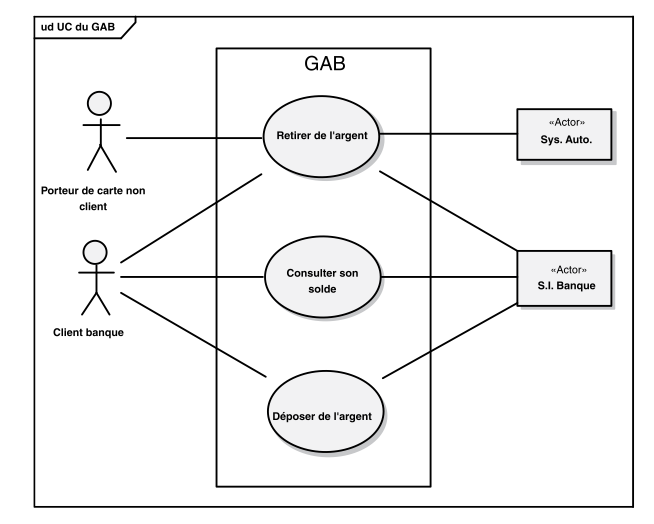
\includegraphics{cas_utilisation} \\
et le textuel:\\

A plus pour de nouvelles aventures feat. \textsc{moi}.
\end{document}